\chapter{Erstellung der Computerspielengines}
\label{chapter:erstellung-der-computerspielengines}

TODO:

\section{Ansatz A: Zufallsauswahl der Spielzüge}
\label{section:erstellung-ansatz-a}

TODO:

\begin{itemize}
    \item generelle Player struktur
    \item TODO: add greedy player as another base comparision
\end{itemize}

\lstinputlisting[
    label={code:random-player},
    caption={Definition des RandomPlayers},
    captionpos=b,
    language=Rust,
    firstline=0,
]{res/code/random-player.rs}

\section{Ansatz B: Principal-Variation-Search}
\label{section:erstellung-ansatz-b}

Verwendung von Negamax Algorithmus (hier phantom moves) (aufruf mit -)
Erweiterung des Alpha-Beta (ref) Generelle struktur Principal Variation search
Iterative Deepening

\ac{PVS}

\subsection{Transposition Table und Zobrist Hashing}

TODO:

\subsection{Aspiration Windows}

TODO:

\subsection{Sucherweiterungen}

TODO:

\subsection{Aktionen-Anordnung}

TODO:

\subsection{Late Move Reduction und Pruning}

\ac{LMR}
\ac{LMP}

TODO:

\subsection{Lazy-SMP}

\ac{SMP}

TODO:

\section{Ansatz C: Monte Carlo Tree Search}
\label{section:erstellung-ansatz-c}

TODO:

\begin{itemize}
    \item Normaler MCTS
    \item UCT (Upper Confidence Bound for Trees)
    \item Parallel (Root und Leaf)
    \item Tree Reuse
    \item Evaluator (WinLoss, Score) -> In Eval genauer betrachten
\end{itemize}

\section{Ansatz D: AlphaZero}
\label{section:erstellung-ansatz-d}

TODO:

\begin{itemize}
    \item Änderungen Gegenüber MCTS / Generelle Funktionsweise
    \item Kodierung des Spielzustandes
    \item Netzwerk-Architektur
    \item Parallelization with Virtual Loss
    \item Training-Loop
\end{itemize}

\subsubsection*{Kodierung des Spielzustandes}

\begin{figure}[!ht]
    \centering
    \vspace*{-1.75cm}
    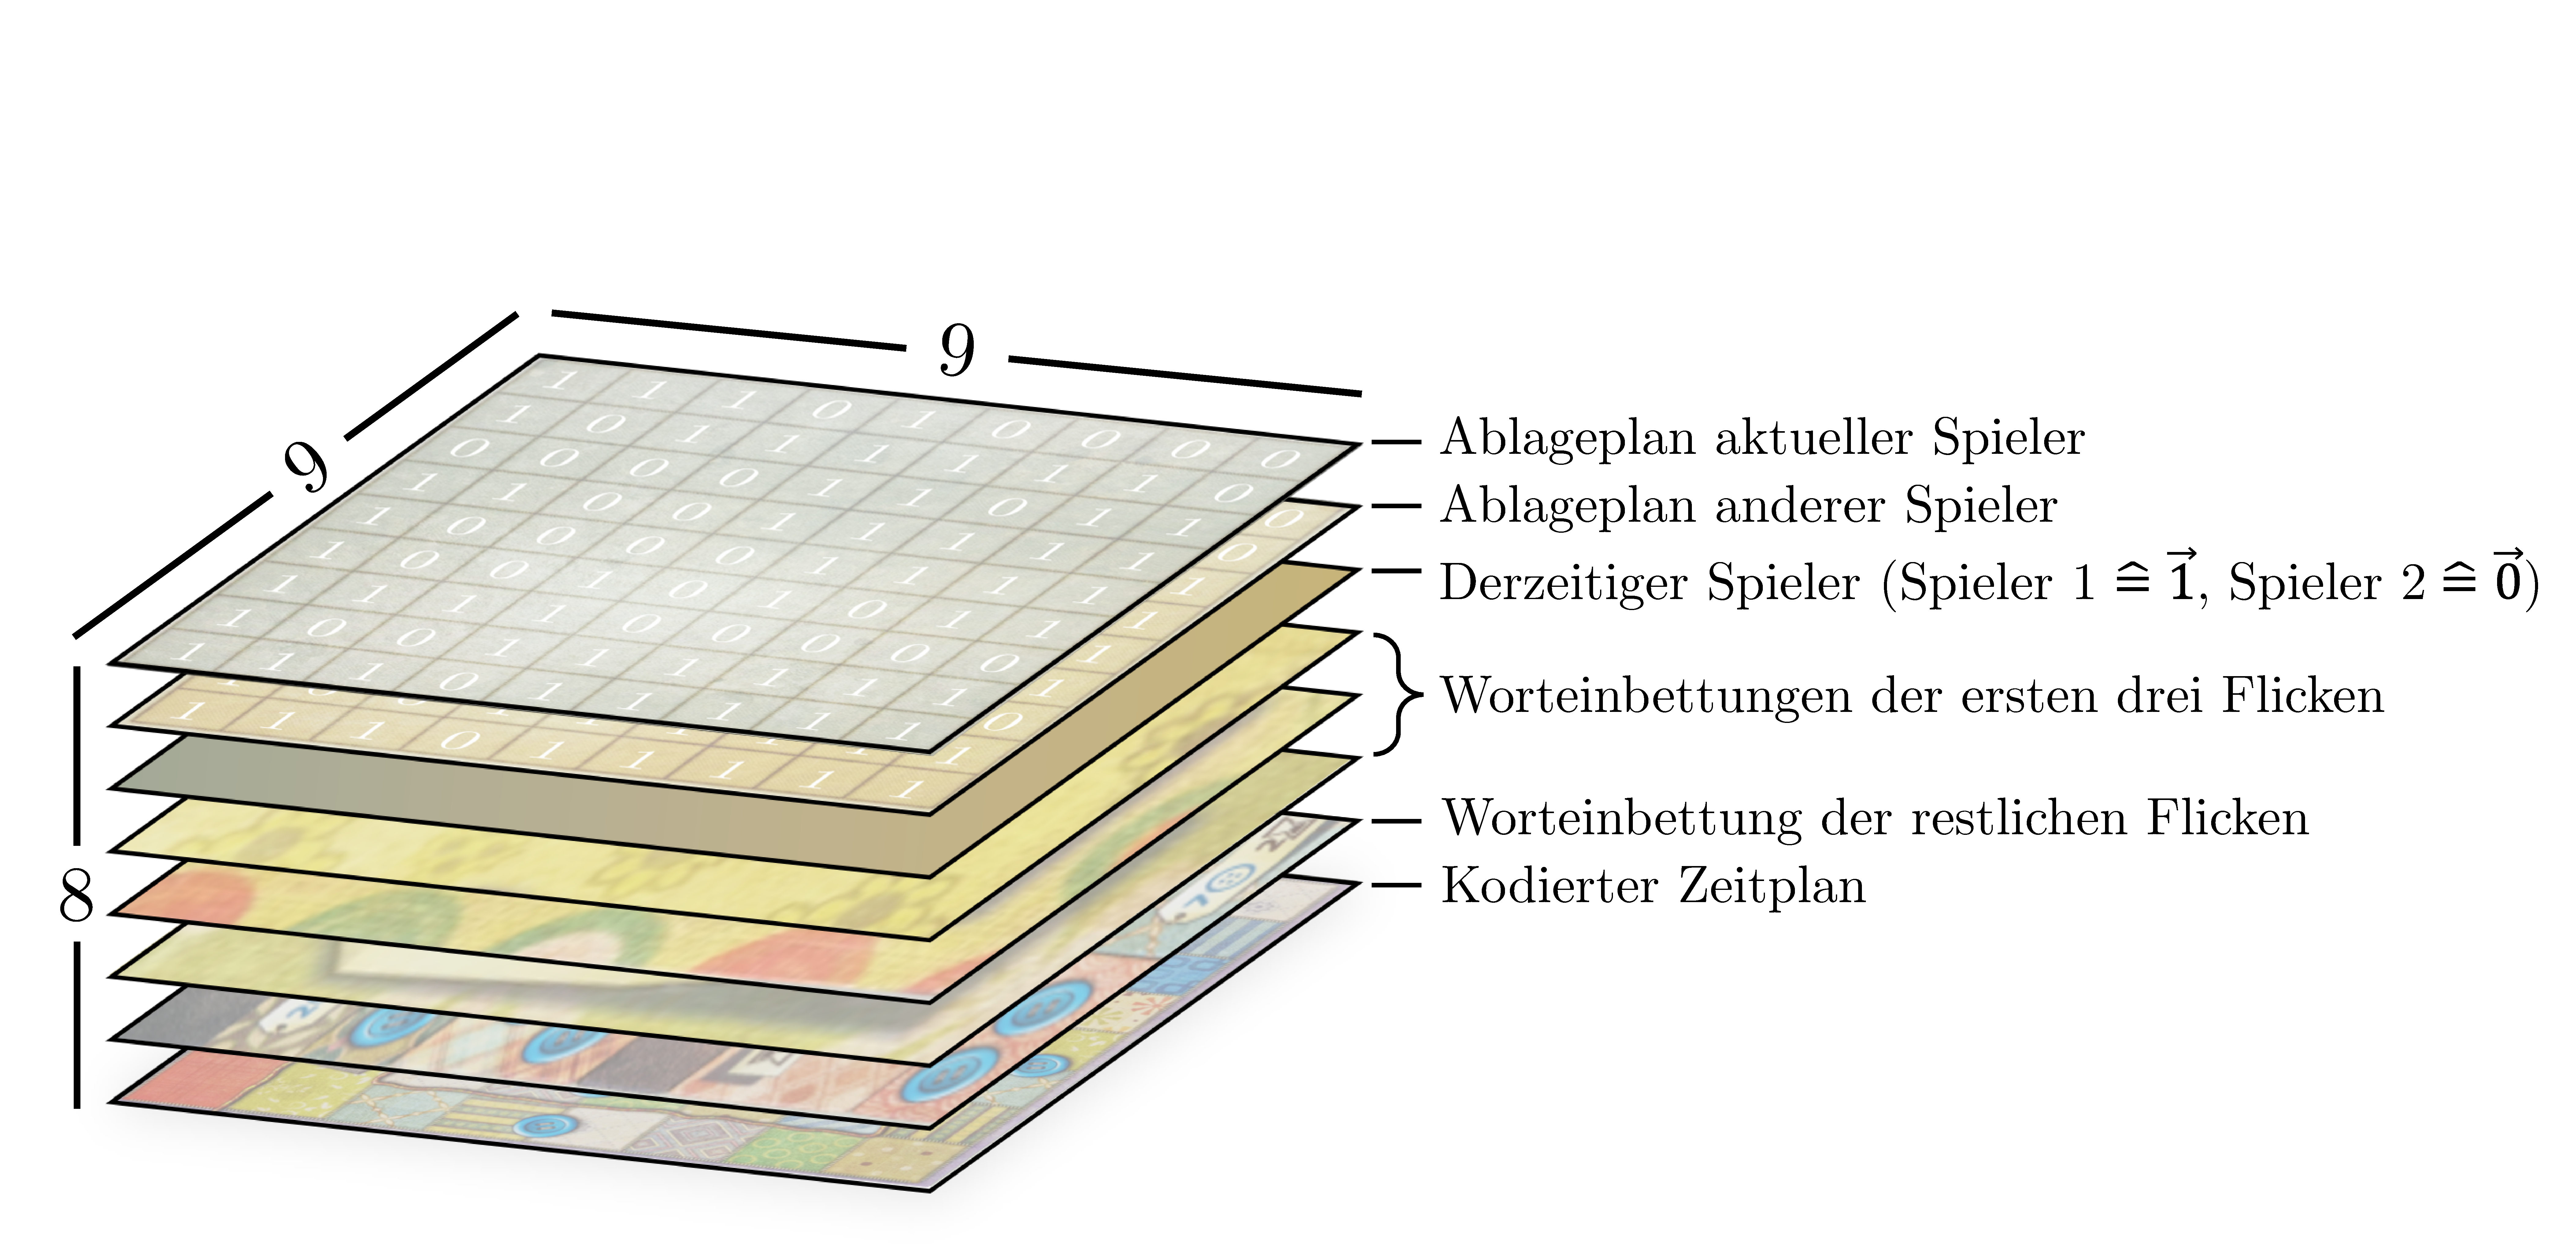
\includegraphics[width=\textwidth]{res/pictures/patch-zero-state.pdf}
    \caption{Zustandskodierung von PatchZero}
    \label{fig:patch-zero-state}
\end{figure}

TODO: LSTM Bild

\pagebreak

\subsubsection*{Netzwerk-Architektur}

\begin{figure}[!ht]
    \centering
    \includegraphics[width=\textwidth]{res/pictures/patch-zero-architecture.pdf}
    \caption{Architektur von PatchZero}
    \label{fig:patch-zero-architecture}
\end{figure}

TODO:

\begin{wrapfigure}{r}{0.25\textwidth}
    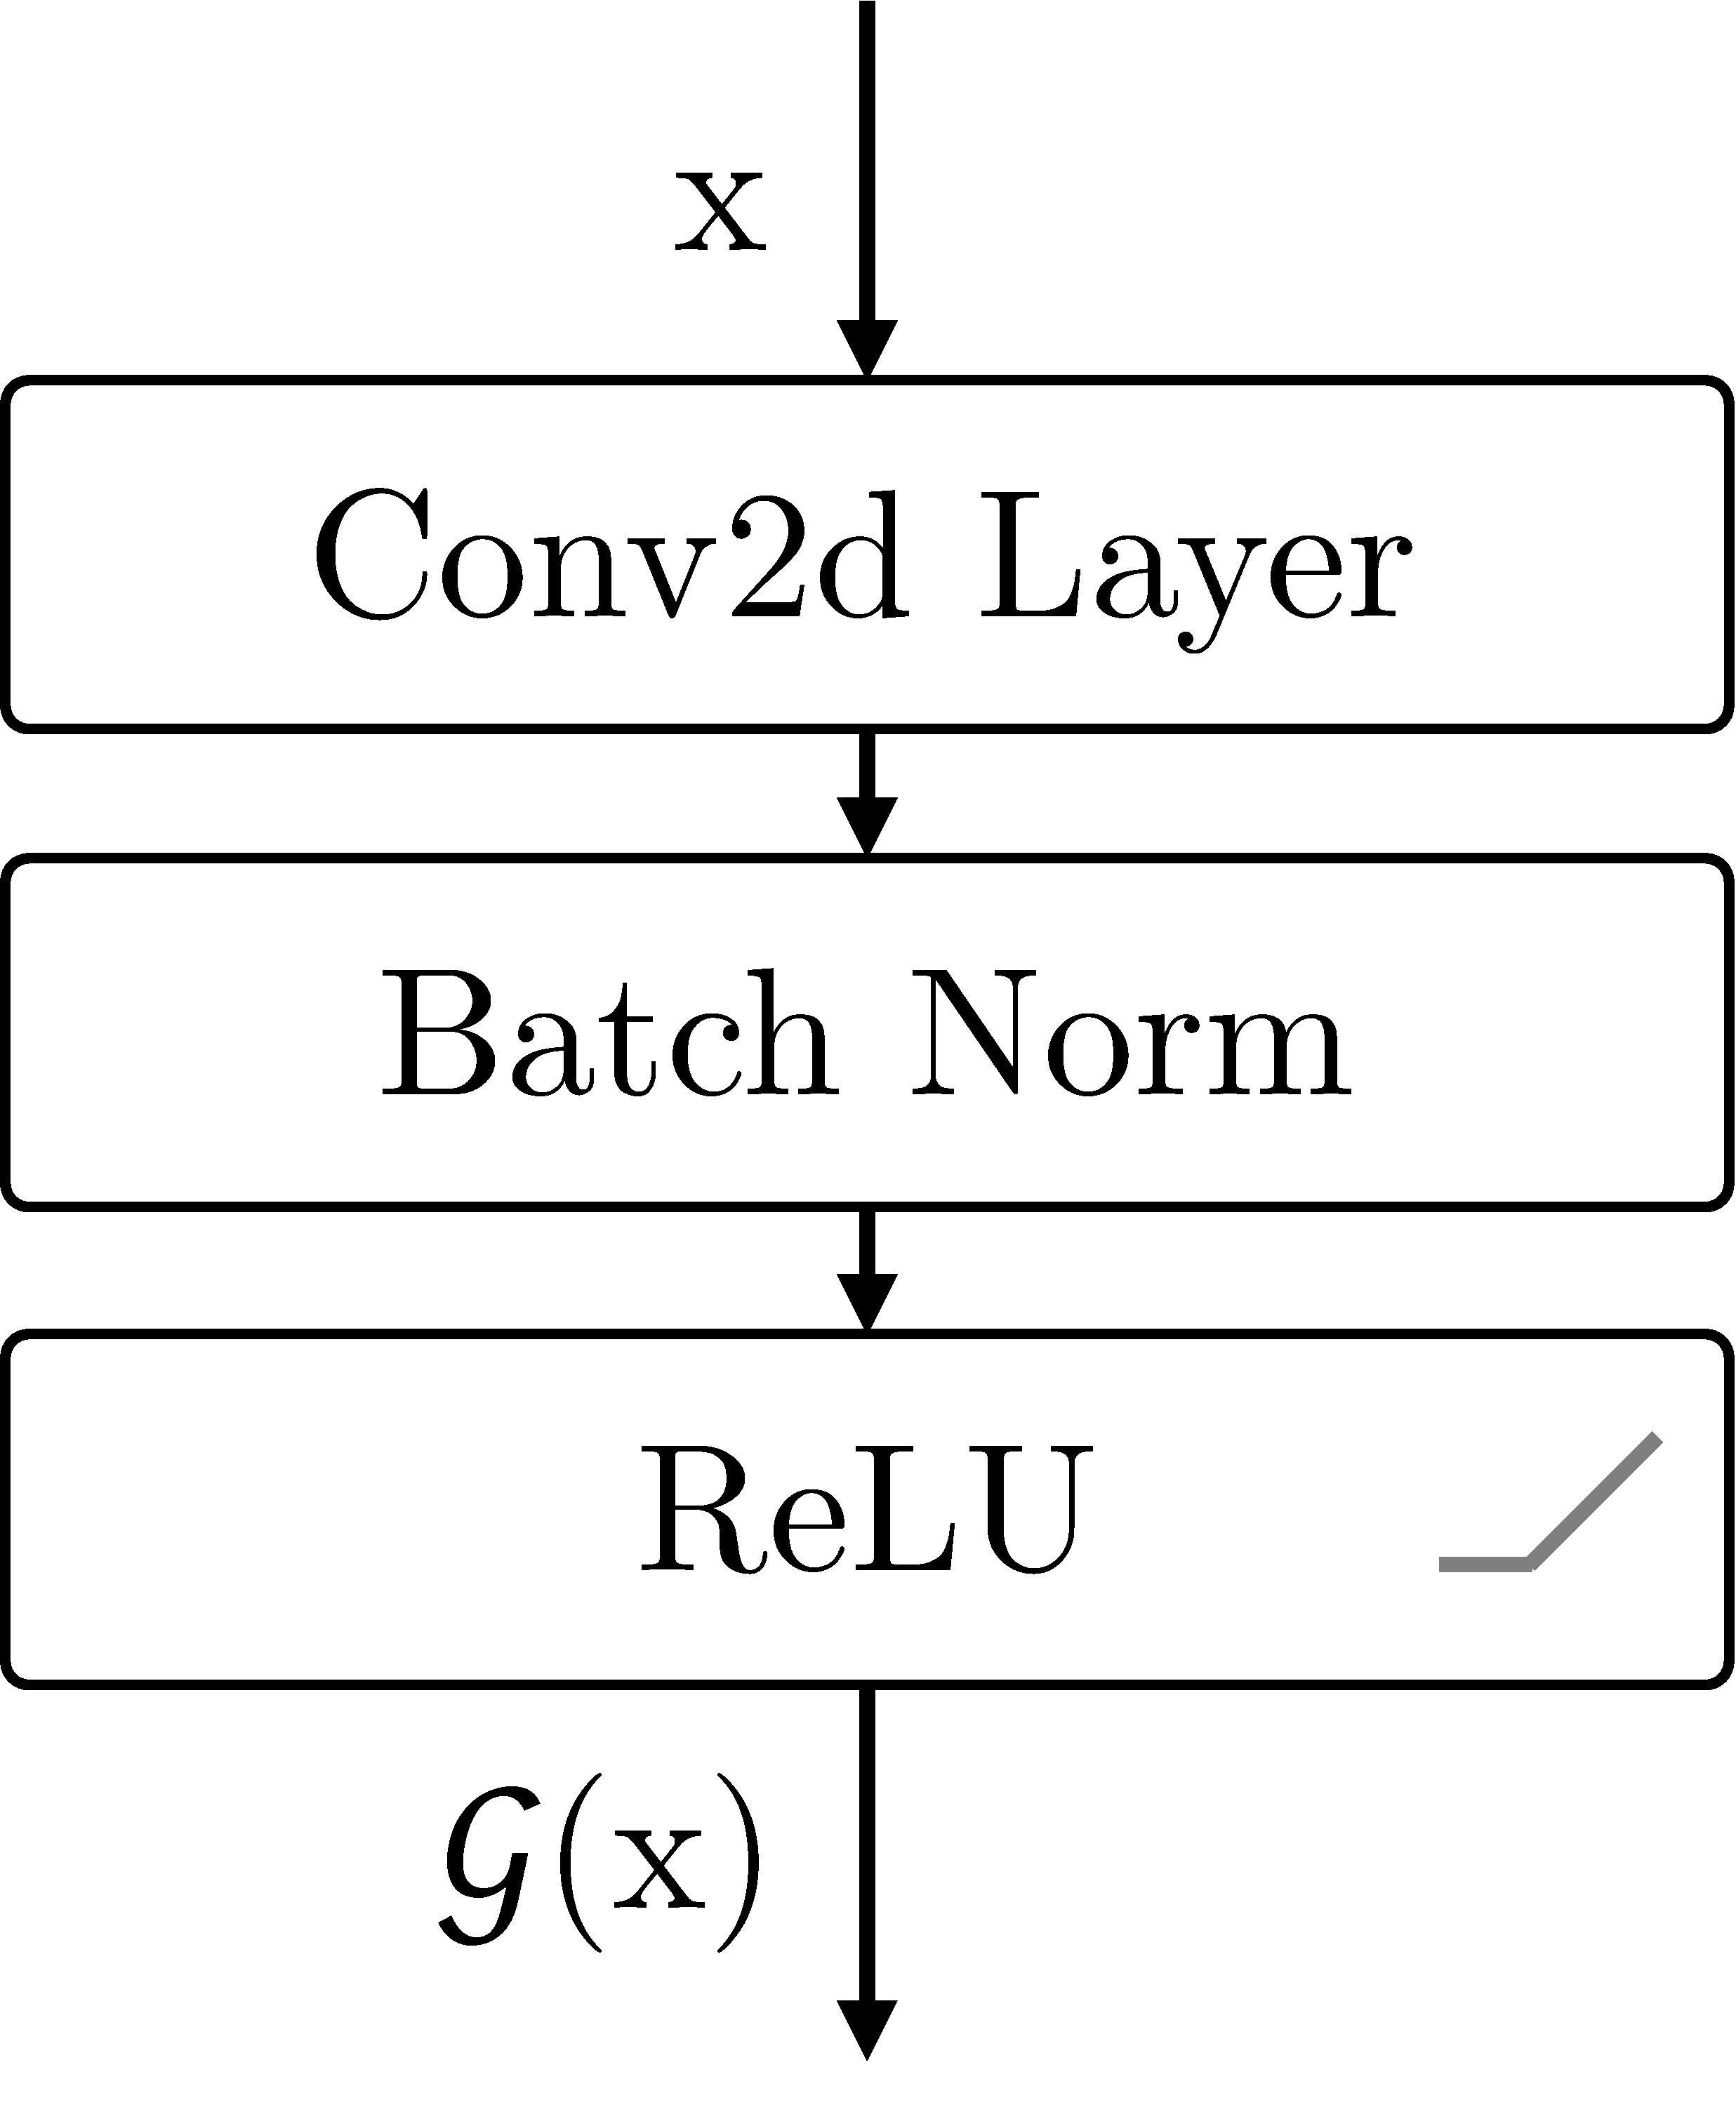
\includegraphics[width=0.2\textwidth]{res/pictures/conv-block.pdf}
    % \vspace{-10pt}
    % Das folgende ist ein Trick, um "Abbilgung x.y" in eine
    % eigene Zeile zu packen. Der Text zwischen [ und ] steht
    % im Abbildungsverzeichnis. Der Text darunter wird
    % tatsächlich angezeigt.
    \centering
    \caption[Convolutional Block]{\unskip}
    Convolutional Block
    \label{fig:conv-block}
\end{wrapfigure}

TODO:

\begin{wrapfigure}{l}{0.3\textwidth}
    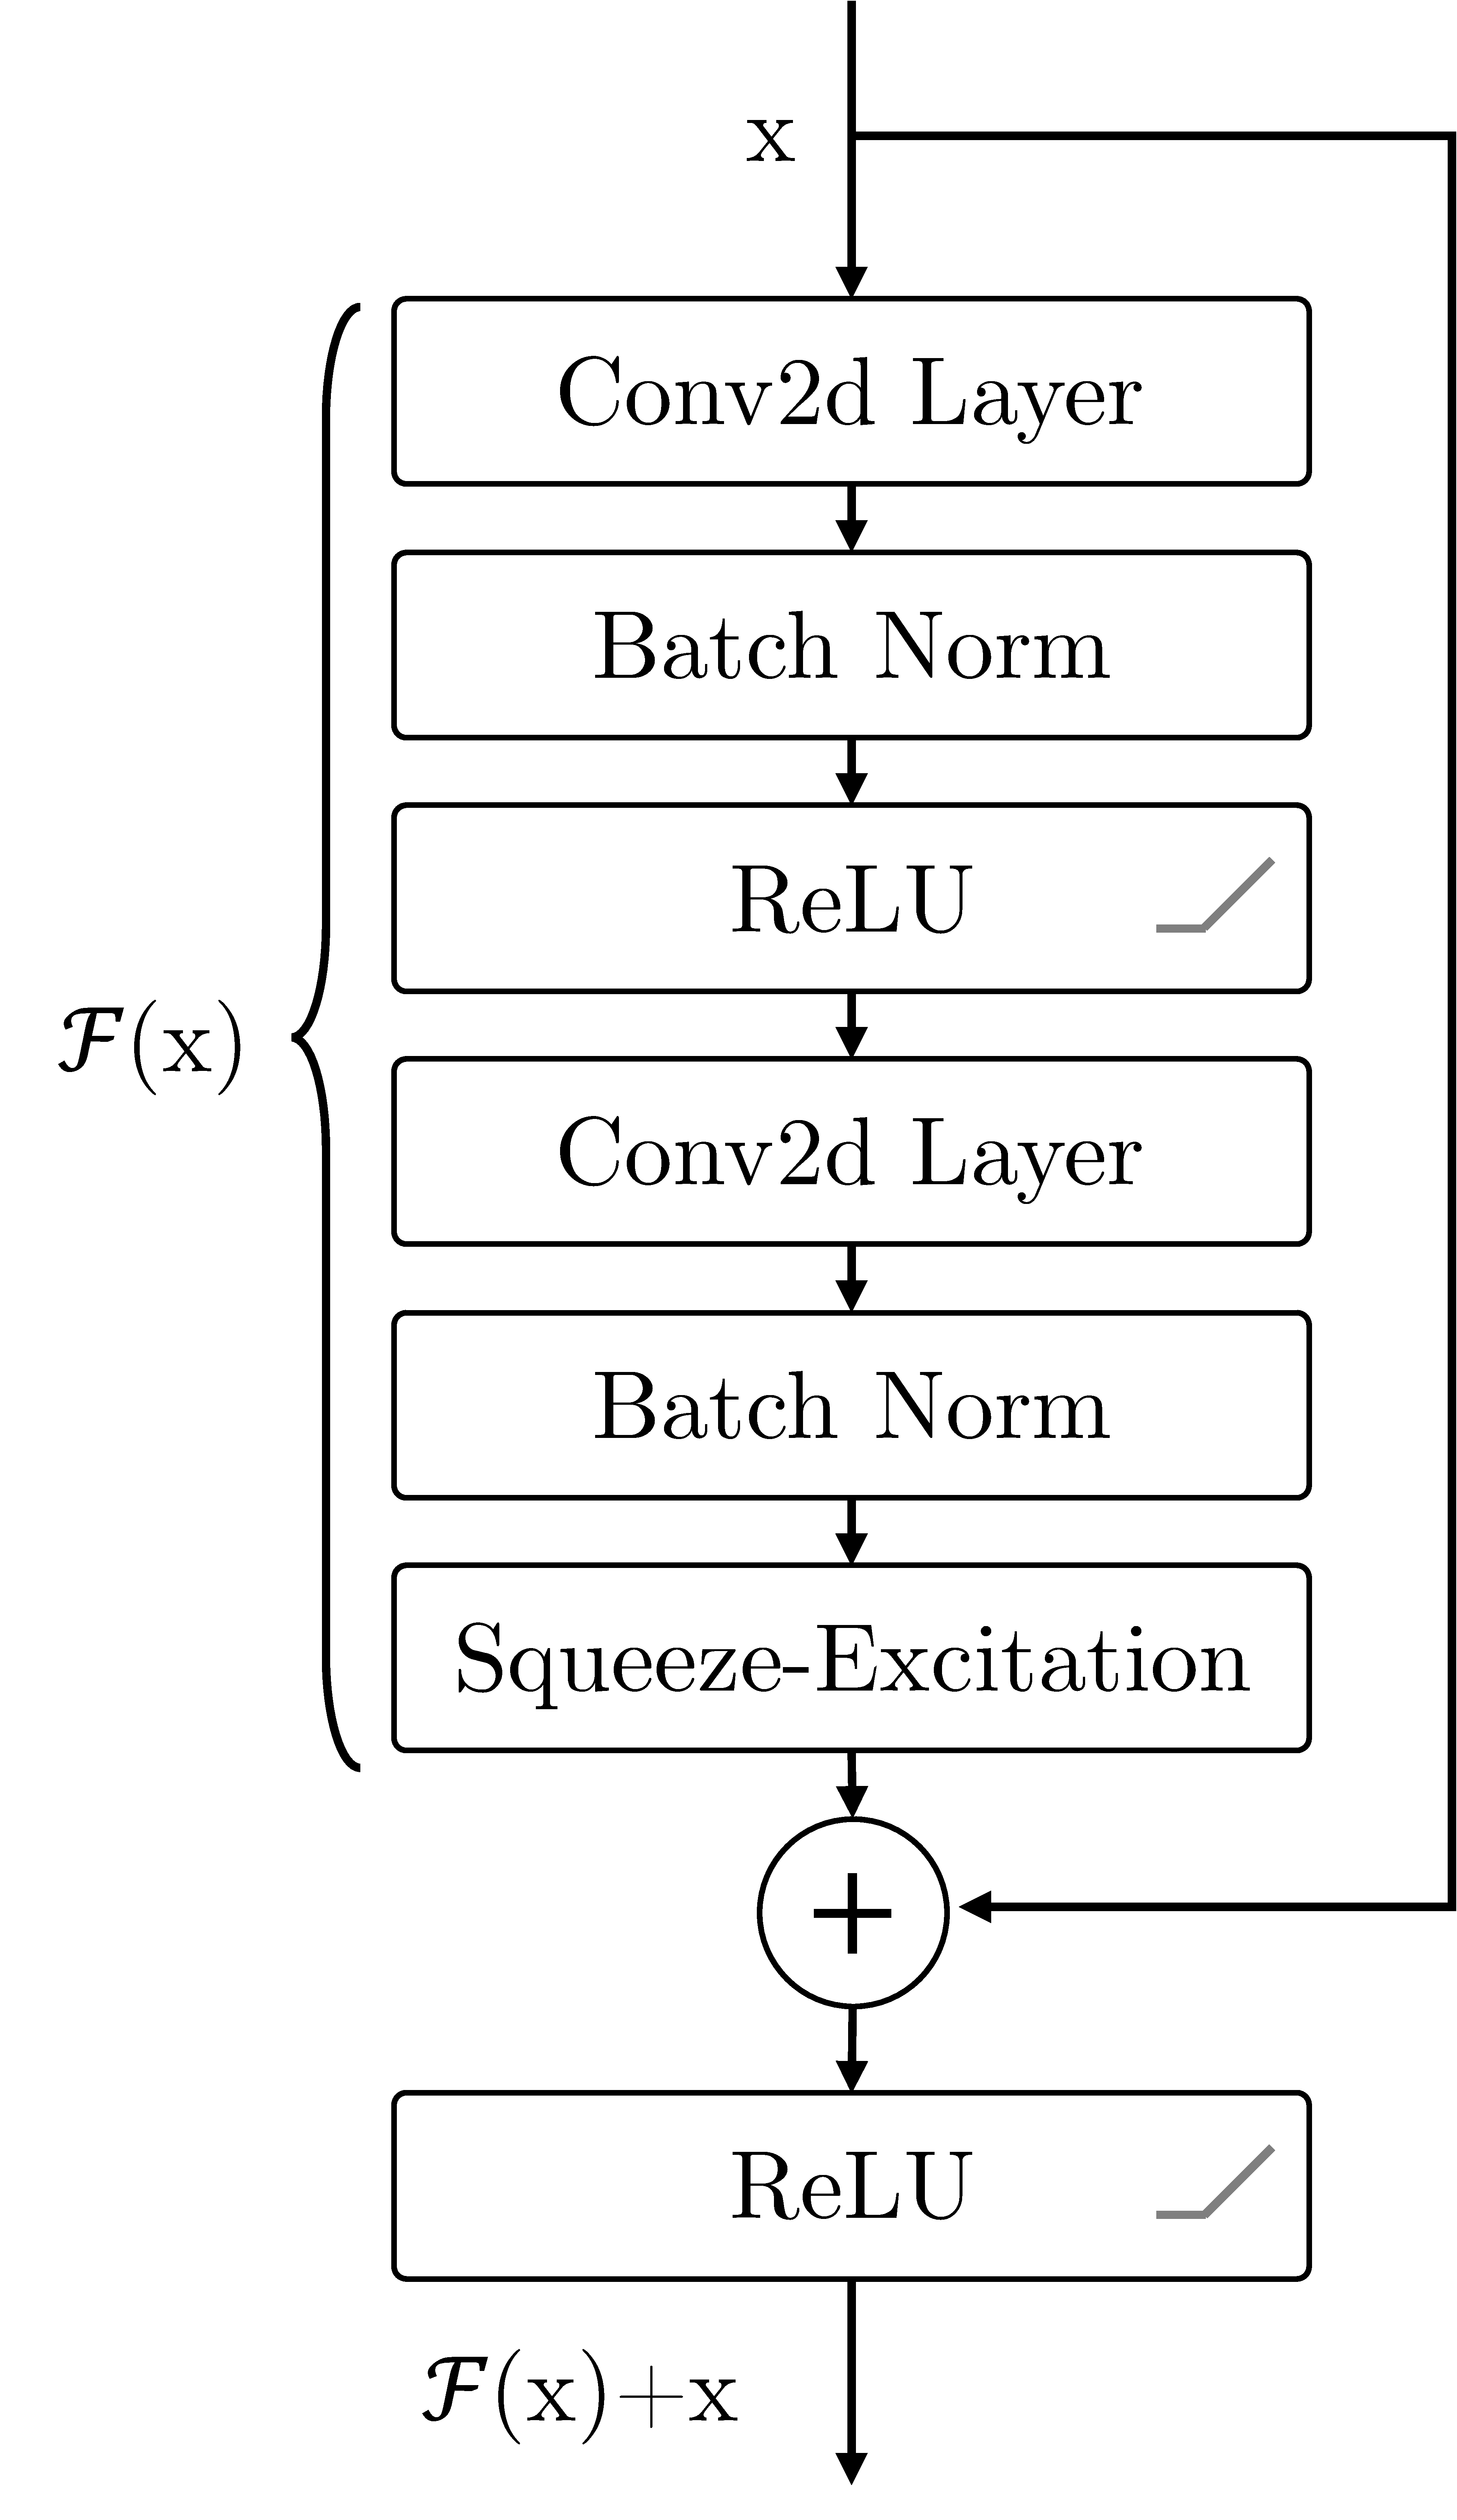
\includegraphics[width=0.25\textwidth]{res/pictures/res-block.pdf}
    % \vspace{-10pt}
    % Das folgende ist ein Trick, um "Abbilgung x.y" in eine
    % eigene Zeile zu packen. Der Text zwischen [ und ] steht
    % im Abbildungsverzeichnis. Der Text darunter wird
    % tatsächlich angezeigt.
    \centering
    \caption[Residual Block]{\unskip}
    Residual Block
    \label{fig:resblock}
\end{wrapfigure}

TODO:

\begin{wrapfigure}{r}{0.35\textwidth}
    \centering
    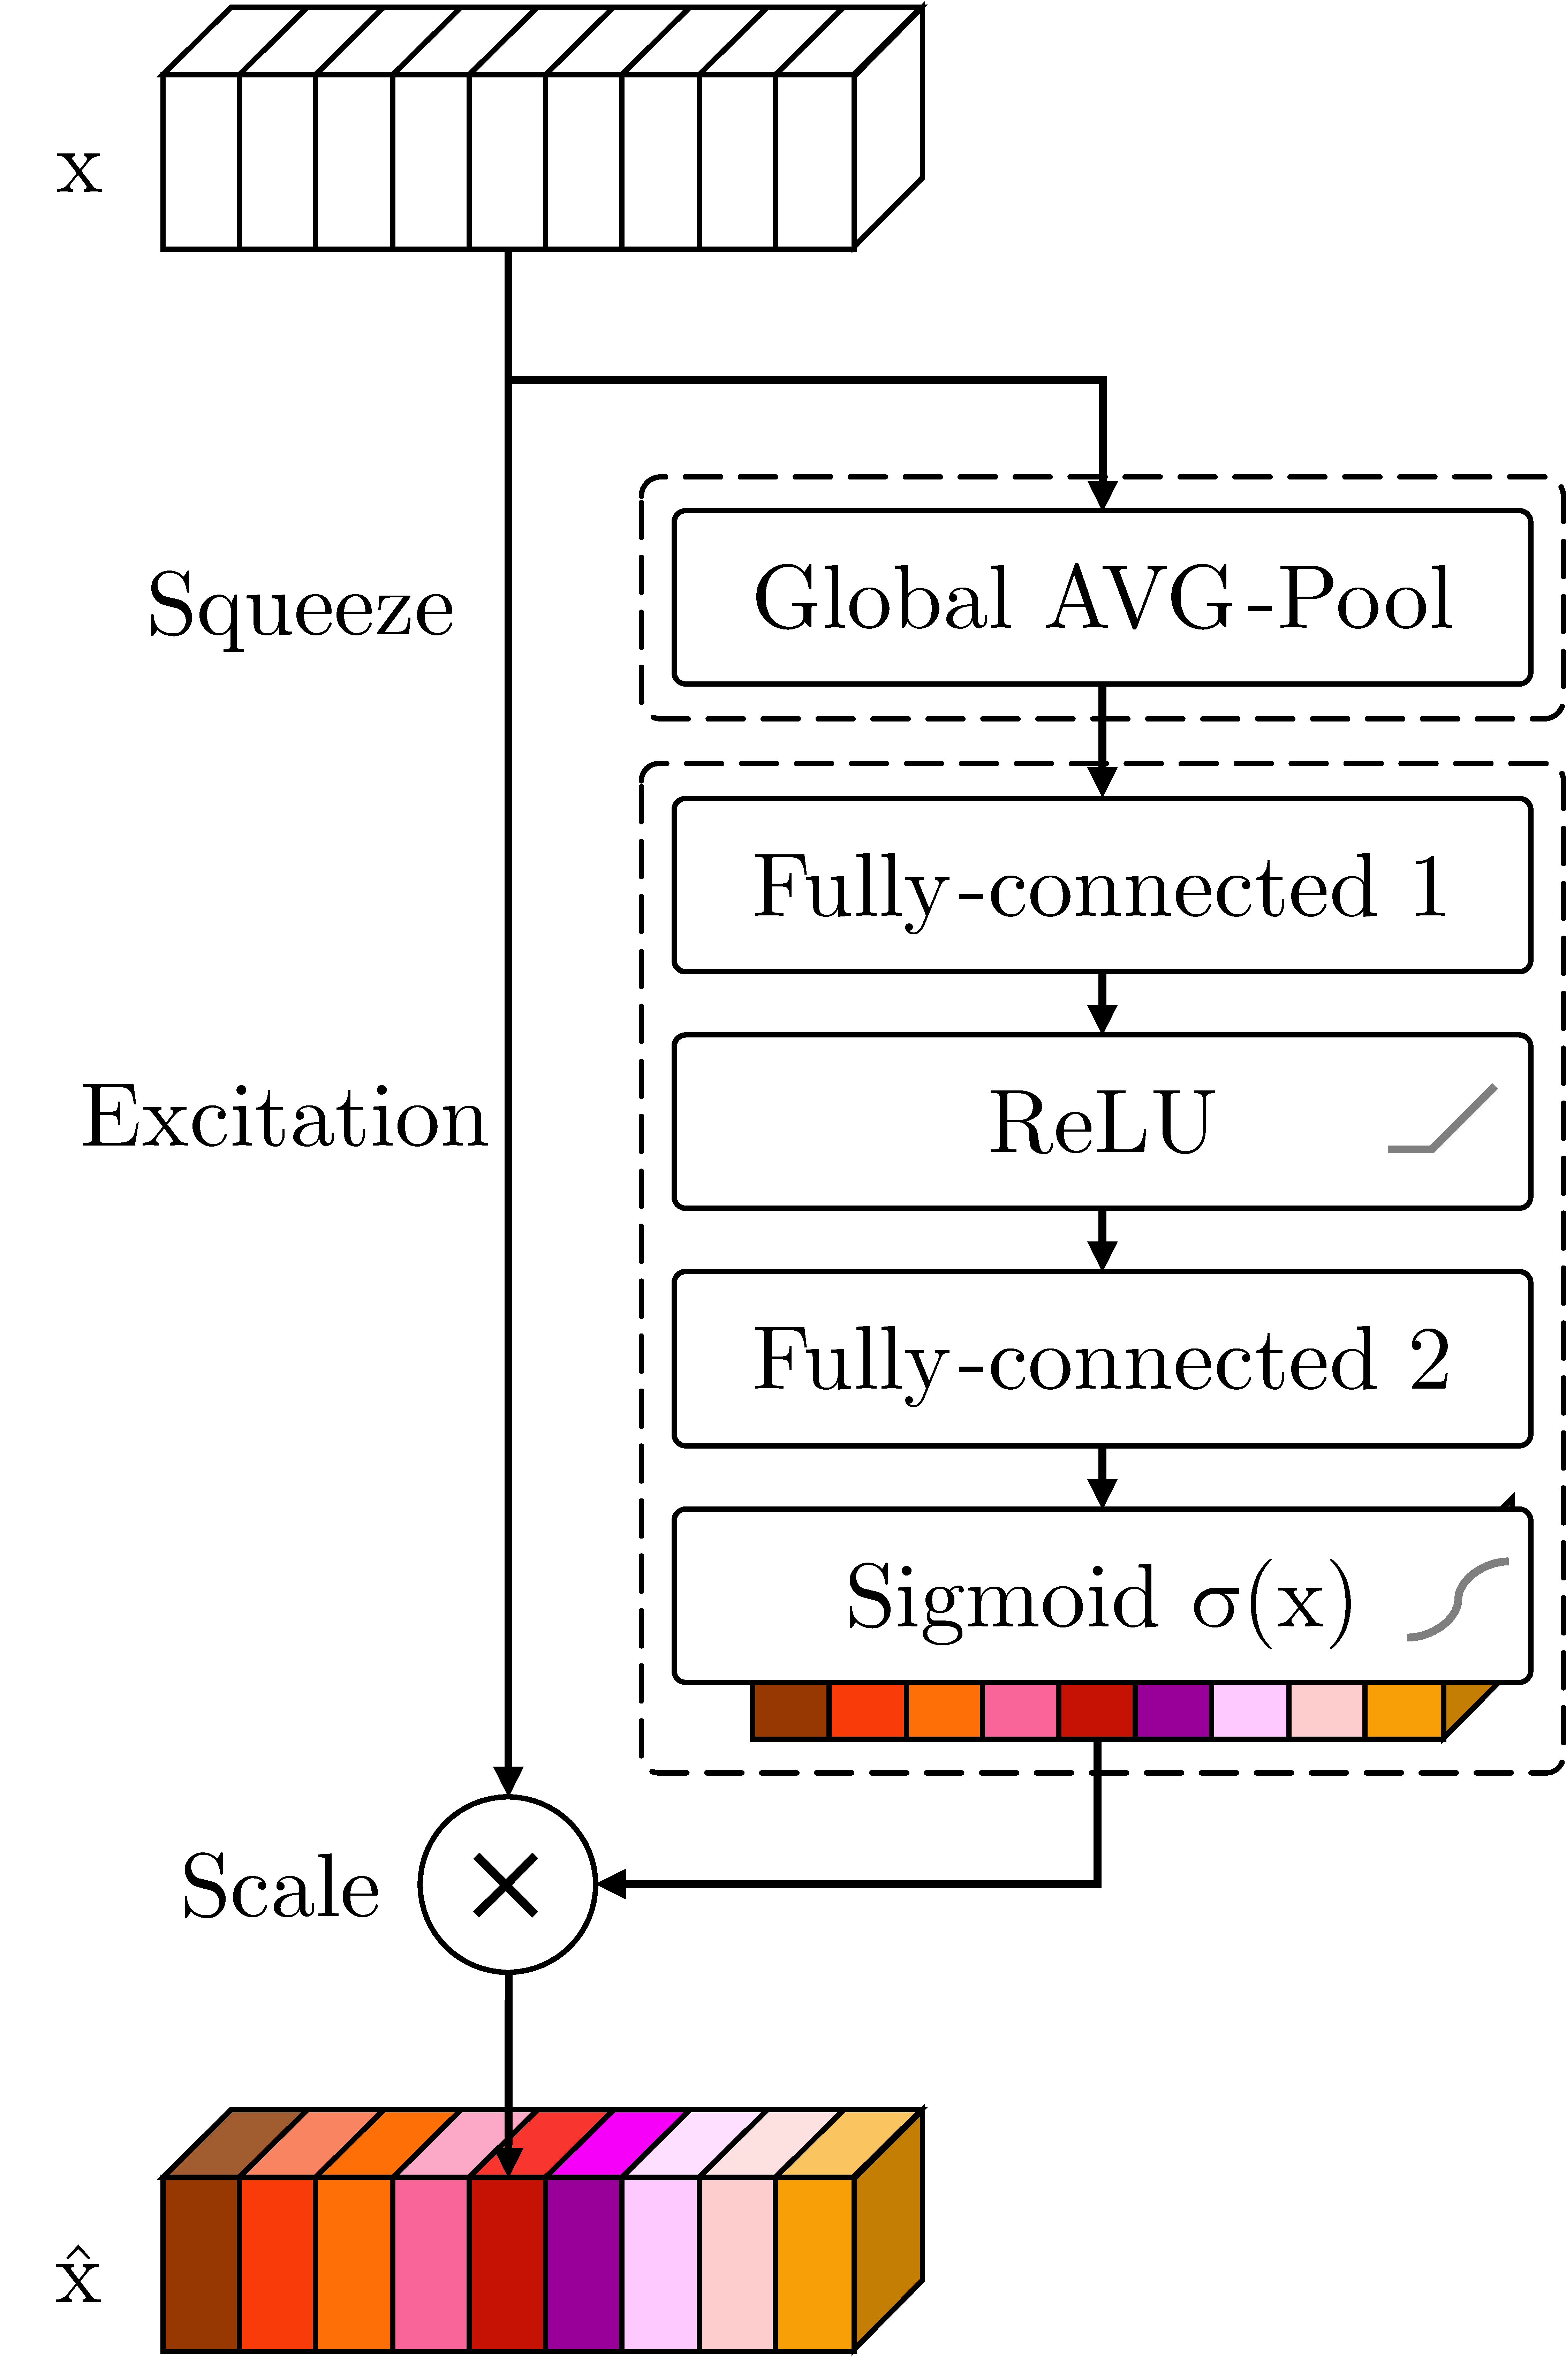
\includegraphics[width=0.3\textwidth]{res/pictures/squeeze-and-excitation-block.pdf}
    % \vspace{-10pt}
    % Das folgende ist ein Trick, um "Abbilgung x.y" in eine
    % eigene Zeile zu packen. Der Text zwischen [ und ] steht
    % im Abbildungsverzeichnis. Der Text darunter wird
    % tatsächlich angezeigt.
    \caption[Squeeze \& Excitation Block]{\unskip}
    Squeeze \& Excitation Block
    \label{fig:squeeze-and-excitation-block}
\end{wrapfigure}

TODO:

\pagebreak

\begin{figure}[!ht]
    \centering
    \includegraphics[width=0.7\textwidth]{res/pictures/value-and-policy-head.pdf}
    \\
    \begin{minipage}{.49\textwidth}
        \centering
        \captionof{figure}[Value Head von PatchZero]{\unskip}
        Value Head von PatchZero
        \label{fig:value-head}
    \end{minipage}
    \hfill
    \begin{minipage}{.49\textwidth}
        \centering
        \captionof{figure}[Policy Head von PatchZero]{\unskip}
        Policy Head von PatchZero
        \label{fig:policy-head}
    \end{minipage}
\end{figure}

TODO: